% ============================================================================ 5 · Expectativas de solución
\section{Expectativas de solución}
\label{sec:solucion}

Ford espera que la solución tenga algún aspecto de por lo menos uno de cuatro campos: análisis de datos,
inteligencia artificial, machine learning o deep learning. La nuestra usa los cuatro:
\begin{itemize}
  \item \textbf{Análisis de datos}: las auditorías de los crudos, el universo y la comparación dentro del
    mercado (§\ref{sec:datos}).
  \item \textbf{Machine learning}: modelos tabulares, de supervivencia en tiempo discreto y de cura, con
    validación agrupada y auditorías de leakage.
  \item \textbf{Deep learning}: el finalista es una red recurrente con atención sobre la secuencia de la ventana.
  \item \textbf{IA generativa}: agentes que redactan los avisos, controlados por un verificador en código.
\end{itemize}

% ---------------------------------------------------------------------------------------------- 5.1
\subsection{Objetivo de mejora: anticipar con el mayor margen posible}
\label{sec:objetivo}

\subsubsection{El recorrido: más de 40 modelos, la misma cuenta}

Probamos de lo simple a lo complejo, y cada familia nos enseñó algo. La tabla~\ref{tab:recorrido} resume el
camino. Las cifras de la entrega 1 no se comparan con las de la v2: la población, las etiquetas y el nulo
cambiaron.

\begin{table}[H]
\centering
\caption{Qué probamos, qué dio y qué aprendimos. Todo es de desarrollo salvo donde dice [test].}
\label{tab:recorrido}
\scriptsize
\begin{tabularx}{\textwidth}{@{}>{\raggedright\arraybackslash}p{3.6cm}>{\raggedright\arraybackslash}p{4.1cm}>{\raggedright\arraybackslash}X@{}}
\toprule
Modelo o idea & Resultado & Qué aprendimos \\
\midrule
\multicolumn{3}{@{}l}{\textbf{Entrega 1} (290 autos de desarrollo, 2 mercados)} \\
Logística y LightGBM sobre 53 features & PR-AUC por debajo del techo de cohorte; \aprime{} del control
  −0,0055 ± 0,0040 & Aprenden \emph{qué auto}, no \emph{cuándo}. Cambiamos la métrica (§\ref{sec:metricas}) \\
Proceso gamma de degradación & No se implementó & No hay carga irreversible medible a estos kilometrajes
  (el 51\,\% de las regeneraciones termina en 0 exacto) \\
Horizonte ordinal (bins) & No reemplaza al binario & Afinar bins no mueve la aguja \\
TimesFM zero-shot (Google) & No le gana a la tasa base & Sugirió medir el desvío respecto de la historia del
  auto; lo medimos y tampoco sumó \\
CNN-LSTM de la tutora & 11,9\,\% ± 3,6 al 5\,\% (3 repeticiones) & Con pocos eventos, las redes no tienen con
  qué aprender \\
Survival stacking (hazard por bin de km) & Único con \aprime{} positivo estable (+0,016 ± 0,003); calibrado
  (Brier 0,112) & Finalista de F3: elegido por \aprime{} y estabilidad, no por PR-AUC \\
Efecto aleatorio por auto (GPBoost) & Pierde contra el apilado simple & El efecto por auto absorbe justo lo que
  distingue autos \\
Cure model por hito post-venta & Señal real (p = 0,005) pero empata con un solo número de uso (km por día) &
  El rasgo temprano existe y es débil \\
K2: survival stacking con la ventana del registro & 17,0\,\% ± 3,8 al 5\,\%; el embolsado, 15,6\,\% &
  Finalista de la entrega 1; el pitch de entonces citaba \textasciitilde15–17\,\% \\
\midrule
\multicolumn{3}{@{}l}{\textbf{Entrega v2} (446 autos de desarrollo, 5 mercados, 135 fallados con cortes)} \\
K2 sin su ventana & Falla \aprime{}; survival stacking detecta \textasciitilde11–14\,\% al 5\,\% & La corrección de
  K2 era la ventana, que en v2 no existe \\
Re-medición de 42 modelos & GRU + viajes + estática ×3: 27 · 42 · 61\,\% al 5 · 10 · 20\,\% & Con 3× los
  eventos, los secuenciales pasan adelante; ninguno le gana con evidencia a la celda \\
Sweep bayesiano de la GRU (130 trials) & El mejor empata con semillas nuevas (0,469 contra 0,471) & La semilla
  mueve más que los hiperparámetros (0,395–0,476): se reporta un ensamble de 3 \\
GRU con etiqueta suave lejos del evento & +9,6 [3,0; 14,4] en dev; −13,3 [−25,0; +3,9] \tagtest{} & Ganaba en dev y
  no se sostuvo (§\ref{sec:suave}) \\
10 semillas y ensambles heterogéneos & Ninguno se mueve más de ±3 puntos al 5–10\,\% & Hay un techo de
  información, no de modelo \\
MiniRocket (kernels aleatorios + ridge) & 16 · 27 · 39\,\% contra 28 · 43 · 61\,\% de la GRU; −16 al 10\,\%
  [−26; −8] & Pierde con evidencia: las convoluciones aprendidas usan mejor la poca señal \\
\bottomrule
\end{tabularx}
\fuente{\repo{decisiones.md} (20-09 a 01-10); \repo{f3-mejor-modelo-a-la-fecha.md};
\repo{f9-remedicion-completa-v2.md}; \repo{f10-sweep-gru.md}; \repo{f11-*.md}; \repo{f12-preregistro-deteccion.md};
MiniRocket: \repo{origin/\allowbreak{}exp/\allowbreak{}minirocket:docs/\allowbreak{}memoria/\allowbreak{}f13-preregistro-minirocket.md}.}
\end{table}

\begin{table}[H]
\centering
\caption{Los modelos principales re-medidos sobre el dev v2 \tagdev{}: detección (\%) con umbral exacto,
promedio de 3 repeticiones; AUC por auto agrupado y dentro de mercado × motor.}
\label{tab:dev}
\small
\begin{tabular}{@{}lrrrrr@{}}
\toprule
Modelo & AUC auto & AUC celda & 5\,\% & 10\,\% & 20\,\% \\
\midrule
\textbf{GRU + viajes + estática ×3 (finalista)} & 0,82 & 0,65 & 27 & 42 & 61 \\
CNN-LSTM + viajes + estática ×3 & 0,81 & 0,62 & 22 & 41 & 62 \\
CNN-LSTM de la tutora + estática ×3 & 0,82 & 0,62 & 27 & 40 & 68 \\
Survival stacking (F3) & 0,72 & 0,57 & 14 & 24 & 42 \\
LightGBM (control, 53 features) & 0,72 & 0,57 & 18 & 28 & 42 \\
Logística L2 & 0,71 & 0,58 & 15 & 23 & 37 \\
\midrule
Celda mercado × motor (sin modelo) & 0,81 & 0,46 & 18 & 33 & 62 \\
Solo el odómetro del corte & 0,42 & 0,43 & 3 & 6 & 15 \\
Azar (puntaje permutado, historial conservado) & — & — & 5 & 11 & 21 \\
\bottomrule
\end{tabular}
\fuente{\repo{docs/\allowbreak{}memoria/\allowbreak{}f9-remedicion-completa-v2.md} (42 modelos, con la tabla completa y las comparaciones pareadas).}
\end{table}

\textbf{La lectura conjunta.} Los secuenciales ordenan autos \emph{dentro} de la celda mercado × motor con
AUC 0,62–0,65, contra 0,57 de survival stacking y de los tabulares, y le ganan a survival stacking con
evidencia entre el 10 y el 20\,\% de falsas alarmas (GRU con estática, +18,8 puntos al 10\,\%, IC95 [9,1; 27,9]).
La celda sola, en cambio, es un piso altísimo: el uso le suma \textasciitilde5–10 puntos al 5–10\,\% y al
20\,\% empata. Con la primera entrega (53 fallados) la CNN-LSTM quedaba por debajo de survival stacking: las
redes necesitaban los datos que trajo la v2.

\subsubsection{El finalista: una red que lee los viajes en orden y recuerda}
\label{sec:gru}

\begin{figure}[H]
\centering
\begin{tikzpicture}[font=\sffamily\scriptsize,
  bin/.style={draw=fordblue!60,fill=softbg,minimum width=6mm,minimum height=9mm,inner sep=0pt},
  cell/.style={draw=fordblue,fill=fordblue!15,rounded corners=2pt,minimum width=7mm,minimum height=6mm},
  blk/.style={draw=inksec,fill=white,rounded corners=2pt,align=center,inner sep=3pt},
  arr/.style={-{Stealth[length=1.6mm]},draw=inksec}]
\foreach \i/\l in {0/1,1/2,2/3,4/20} {
  \node[bin] (b\i) at (\i*1.05,0) {\l};
  \node[cell] (h\i) at (\i*1.05,1.25) {$h_{\l}$};
  \draw[arr] (b\i) -- (h\i);
}
\node at (3*1.05,0) {\dots}; \node at (3*1.05,1.25) {\dots};
\draw[arr] (h0) -- (h1); \draw[arr] (h1) -- (h2); \draw[arr] (h2) -- ++(0.6,0); \draw[arr] (3.5,1.25) -- (h4);
\node[below=1mm of b2,align=center,text width=5.2cm] {20 tramos de 50 km (los últimos 1.000 km) ×
  15 canales: cómo se viaja y qué hace el filtro};
\node[blk,above=6mm of h2,text width=3.6cm] (att) {\textbf{Atención}: un peso por tramo y el promedio pesado de
  las 20 memorias};
\foreach \i in {0,1,2,4} {\draw[arr,muted] (h\i) -- (att);}
\node[blk,left=10mm of att,text width=3cm] (st) {\textbf{País, motor y serie}\\(rama estática de 4)};
\node[blk,above=6mm of att,text width=3.6cm] (head) {\textbf{Cabeza} (16) → puntaje de riesgo a 3.000 km};
\draw[arr] (att) -- (head); \draw[arr] (st) |- (head);
\node[blk,right=6mm of head,text width=3.2cm,draw=accent2!80,fill=warnbg] (ens) {\textbf{3 redes} (semillas 42, 1, 2)
  votan por rango};
\draw[arr] (head) -- (ens);
\node[right=2mm of h4,align=left,text width=3.4cm,inksec] {GRU unidireccional, memoria de 24 números; dos
  compuertas deciden qué anotar y qué olvidar en cada tramo};
\end{tikzpicture}
\caption{La GRU finalista. Unos 3.900 parámetros: GRU 2.952, atención 416, rama estática 52 y cabeza 481.}
\label{fig:gru}
\fuente{\repo{src/\allowbreak{}models/\allowbreak{}gru\_seq.py}; \repo{configs/\allowbreak{}exp\_v2all\_gru\_trips\_estaticas\_r3.yaml};
\repo{docs/\allowbreak{}pitch/\allowbreak{}presentacion-contenido.md} (“La GRU por dentro”).}
\end{figure}

\begin{itemize}
  \item \textbf{Qué lee.} Cada 500 km, los últimos 1.000 km del auto en 20 tramos de 50 km. Cada tramo trae 15
    señales: 6 de cómo se viaja (cantidad de viajes, ralentí, viajes que no llegan a temperatura, velocidad, km
    y duración por viaje) y 9 de qué hace el filtro (registros, cobertura, acumulación media y máxima, cuánto
    sube, caídas por regeneración y tres tipos de aviso). Se imputan y estandarizan con el train de cada fold.
  \item \textbf{Cómo recuerda.} Una GRU de una capa, unidireccional, con una memoria de 24 números que se
    actualiza tramo a tramo. La \emph{compuerta de actualización} decide qué parte de la memoria se reemplaza
    con lo nuevo, y la \emph{de reinicio}, cuánto del pasado se usa para armar ese candidato. Así ve
    tendencias que un promedio de los 1.000 km borra: que el hollín viene subiendo o que los viajes se vienen
    acortando. No lee al revés: el estado en el km 200 nunca depende del km 900.
  \item \textbf{Qué mira al final.} Una capa de atención pesa los 20 tramos y arma un resumen. Se le suman país,
    motor y serie por una rama estática chica, y una cabeza da el puntaje.
  \item \textbf{Cómo aprende.} Con la etiqueta dura (1 si el evento cae entre 500 y 3.500 km después del corte),
    sobre las \textasciitilde11.700 filas de desarrollo. La pérdida pesa más los positivos (negativos sobre
    positivos del train). Adam con tasa 0,001, weight decay 1e-4, recorte del gradiente en 1,0, dropout 0,3, 40
    épocas fijas, lote de 64, en CPU. Sin early stopping: el modelo no conoce el vehículo, así que no puede
    apartar una validación agrupada propia.
  \item \textbf{Por qué chica.} Con 135 autos que fallan para aprender, una red más grande memoriza autos en vez
    de hábitos. La GRU tiene una compuerta menos que una LSTM, y por eso menos parámetros para la misma tarea.
  \item \textbf{Ensamble.} Tres redes con semillas distintas (42, 1 y 2); se promedia el rango de cada una. Las
    semillas son las del reporte v2 y no se eligieron por resultado. La alerta salta con dos cortes seguidos
    sobre el umbral.
  \item \textbf{Nadie le explicó el filtro.} La relación entre viajes cortos y hollín la encontró en los datos
    (§\ref{sec:explicabilidad}).
\end{itemize}

\subsubsection{El resultado, en autos que nunca vio}
\label{sec:test}

El test son los 111 autos del holdout. 103 tienen cortes en el panel: 32 fallaron y 71 no. Cada modelo se
entrenó con todo el desarrollo (446 autos) y se midió una vez con la misma cuenta que en dev
(\repo{scripts/\allowbreak{}eval\_test.py}).

\begin{figure}[H]
\centering
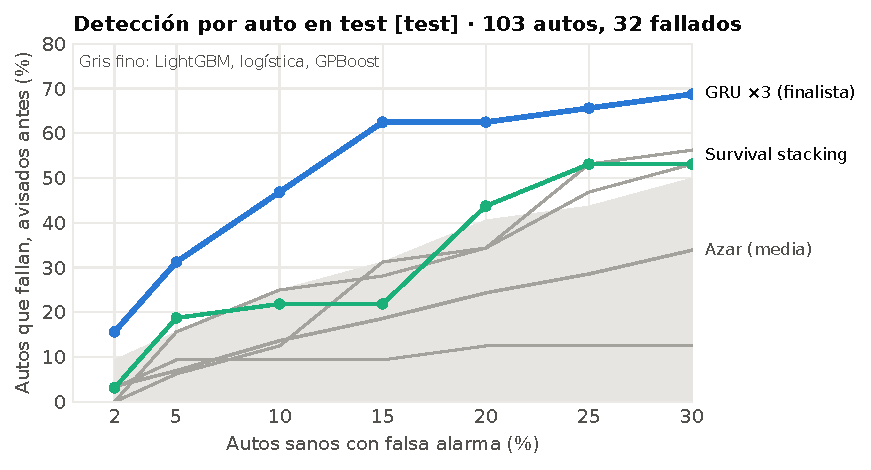
\includegraphics[width=\textwidth]{figuras/curva_test.pdf}
\caption{Detección de autos que fallan según el porcentaje de sanos con falsa alarma, en test. La banda gris
es el azar hasta su percentil 95. La celda mercado × motor no detecta nada por debajo del 10\,\% porque alerta
celdas enteras.}
\label{fig:curva}
\fuente{\repo{experiments/\allowbreak{}test-modelos-v2/\allowbreak{}curve.csv} (\repo{configs/\allowbreak{}eval\_test\_modelos\_v2.yaml}); figura:
\repo{scripts/\allowbreak{}make\_report\_figures.py}.}
\end{figure}

\begin{table}[H]
\centering
\caption{El finalista en test \tagtest{}: detección (\%) por presupuesto de falsas alarmas.}
\label{tab:test}
\small
\begin{tabular}{@{}lrrrrr@{}}
\toprule
 & 5\,\% & 10\,\% & 15\,\% & 20\,\% & Primario (5–20\,\%) \\
\midrule
\textbf{GRU ×3 (semillas 42, 1, 2)} & \textbf{31,2} & \textbf{46,9} & \textbf{62,5} & \textbf{62,5} & \textbf{50,8} \\
Survival stacking (finalista de la entrega 1) & 18,8 & 21,9 & 21,9 & 43,8 & 26,6 \\
Celda mercado × motor (sin modelo) & 0,0 & 21,9 & 21,9 & 50,0 & 23,4 \\
Azar, media & 7,0 & 13,7 & 18,6 & 24,4 & — \\
Azar, p95 & 15,6 & 25,0 & 31,2 & 40,6 & — \\
\bottomrule
\end{tabular}
\fuente{\repo{experiments/\allowbreak{}test-f10-s42/\allowbreak{}report.json}, \repo{experiments/\allowbreak{}test-modelos-v2/\allowbreak{}report.json};
\repo{docs/\allowbreak{}memoria/\allowbreak{}f11-test-resultado.md}. Todos los modelos, en el Anexo~\ref{anx:modelos}.}
\end{table}

\begin{itemize}
  \item \textbf{10 de 32 al 5\,\%: casi uno de cada tres}, 4,5 veces el azar y por encima de su p95. Al 20\,\%,
    seis de cada diez.
  \item \textbf{Le duplica el primario a los tabulares y a survival stacking} (50,8 contra 21–27). Contra survival
    stacking, +24,2 puntos, IC95 [0,8; 43,0]: el intervalo apenas no cruza el cero, y la comparación no estaba
    preregistrada.
  \item \textbf{Contra la celda mercado × motor: +27,3 puntos, IC95 [−0,8; 46,1]}, p(diferencia ≤ 0) = 0,028.
    Queda en el límite y \emph{no} lo citamos como “le gana”.
  \item \textbf{Ordena autos}: AUC por auto 0,794; dentro de mercado × motor, 0,675. Entre autos del mismo país y
    motor, el orden es moderado.
  \item \textbf{Repitió lo de dev}: en validación cruzada daba 27,4 · 42,5 · 53,3 · 60,7\,\% (primario 46,0).
\end{itemize}

\begin{table}[H]
\centering
\caption{El punto de operación con el umbral fijado en dev \tagtest{}: se elige el umbral con los sanos de
desarrollo (15 modelos de fold) y se mide en test cuántas fallas detecta y cuántas falsas alarmas produce de
verdad.}
\label{tab:operacion}
\small
\begin{tabular}{@{}lll@{}}
\toprule
Modelo & Detección (\%) al 5 · 10 · 20\,\% & Falsas alarmas reales (\%) \\
\midrule
GRU ×3 (finalista) & 20 · 34 · 57 & 5,8 · 8,9 · 18,2 \\
Survival stacking & 13 · 20 · 33 & 4,6 · 8,3 · 15,6 \\
LightGBM (53 features) & 16 · 25 · 36 & 7,5 · 10,7 · 16,9 \\
Logística L2 (53 features) & 12 · 16 · 33 & 8,8 · 11,8 · 18,3 \\
SS + efecto aleatorio (GPBoost) & 8 · 11 · 14 & 6,5 · 11,3 · 21,5 \\
\bottomrule
\end{tabular}

\fuente{\repo{experiments/\allowbreak{}test-modelos-v2/\allowbreak{}operating.csv}.}
\end{table}

\textbf{El número para operar.} En producción el umbral no se puede elegir mirando los autos que se quieren
puntuar. Fijado con los sanos de desarrollo, la GRU detecta 20 · 34 · 57\,\% al 5 · 10 · 20\,\% con
\textbf{5,8 · 8,9 · 18,2\,\% de falsas alarmas reales}: el umbral cumple su presupuesto en autos nuevos
(tabla~\ref{tab:operacion}).

\begin{caja}[title={Por qué citamos un rango y no un número}]
\small
La configuración de la GRU se leyó tres veces en test: con las semillas 42/1/2 el 27-09 (34 · 41 · 63\,\% al
5 · 10 · 20\,\%), con las semillas 101–103 como referencia del tiro de F11 (28 · 50 · 50\,\%), y con 42/1/2 el
01-10 (31 · 47 · 63\,\%). La primera lectura fue antes del preregistro de F11 y no pudo inflar ese resultado,
pero el test ya se había mirado. Además, la GRU no es reproducible bit a bit entre corridas, aun con la misma
semilla (correlación 0,88–0,91 entre los puntajes de dos corridas con la misma configuración). Con 32 fallas,
cada auto mueve 3 puntos. Por eso: \textbf{\textasciitilde30\,\% al 5\,\%, \textasciitilde40–50\,\% al 10\,\% y
\textasciitilde50–60\,\% al 20\,\%.}

\textbf{Sin los 36 autos de test que estaban en el desarrollo de la entrega 1} (71 autos, 22 fallados): 36,4 ·
50,0 · 50,0 · 59,1\,\% al 5 · 10 · 15 · 20\,\% (primario 48,9). Lo aprendido mirando la entrega 1 no está
inflando el test.
\fuente{\repo{docs/\allowbreak{}memoria/\allowbreak{}f11-test-resultado.md} §2 y resumen.}
\end{caja}

\subsubsection{Cuánto antes: el margen medido}
\label{sec:anticipacion}

Este es el objetivo de mejora de la sección 5.1 del desafío: anticipar con la mayor cantidad de tiempo o
kilometraje posible.

\begin{itemize}
  \item \textbf{Al 10\,\% de falsas alarmas} \tagtest{}, la primera alerta llega con una mediana de
    \textbf{4.646 km} (p25–p75: 2.403–9.263 km) antes del evento, y unos \textbf{99 días} aproximados con los km
    por día de cada auto. Al 5\,\%: 3.987 km, \textasciitilde72 días. Al 20\,\%: 5.969 km, \textasciitilde109 días.
  \item \textbf{En dev} \tagdev{}, al 10\,\%: mediana \textasciitilde7.600 km (p25–p75: 3.700–13.100), \textasciitilde86
    días. En km el test da menos porque sus autos detectados andan menos km por día; en días es parecido.
    Sin los autos vistos en la entrega 1, la mediana en test es de \textasciitilde8.800 km.
  \item \textbf{El piso es el gap}: por construcción, ninguna alerta usa los 500 km previos al evento. La distancia
    se mide hasta la referencia del evento (fecha registrada − 21 días); hasta la fecha registrada, el margen es
    algo mayor.
\end{itemize}

\begin{figure}[H]
\centering
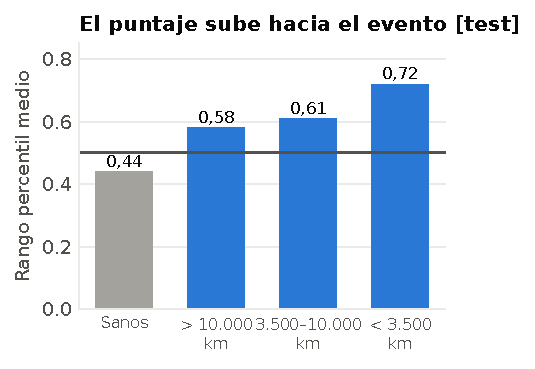
\includegraphics[width=0.62\textwidth]{figuras/score_evento.pdf}
\caption{Rango percentil medio del puntaje en los cortes de autos que fallan, según la distancia al evento, y en
los sanos. El fallado ya está por encima de los sanos lejos del evento (\emph{qué auto}) y sube al acercarse
(algo de \emph{cuándo}).}
\label{fig:score}
\fuente{\repo{docs/\allowbreak{}memoria/\allowbreak{}f11-test-resultado.md} §4 (test, promedio de las 3 semillas).}
\end{figure}

\textbf{Cómo se lee el margen.} El puntaje sube a medida que se acerca el evento (figura~\ref{fig:score}), y la
primera alerta cae a mitad del historial, no en el primer corte: hay algo de \emph{cuándo}. Pero la dispersión es
enorme, y la auditoría \aprime{} del finalista da +0,001 (§\ref{sec:limites}). Por eso la frase defendible es
“\emph{lo marcamos con unos tres meses de margen}”, nunca “\emph{predecimos que falla en tres meses}”.

\subsubsection{Una variante que ganaba en desarrollo y no se sostuvo}
\label{sec:suave}

Es el aprendizaje metodológico más importante del proyecto. Con la etiqueta dura, un corte a 10.000 km del
evento de un auto que falla se entrena igual que uno de un auto sano, aunque la detección se cuente por auto. La
variante F11 entrenaba esos cortes lejanos con 0,15 en vez de 0 (una etiqueta suave).

\begin{itemize}
  \item \textbf{En desarrollo ganaba con evidencia}, en una confirmación preregistrada con folds y semillas
    nuevos: +9,6 puntos de primario, IC95 [3,0; 14,4], p = 0,0015 (34,6 · 48,6 · 60,2 · 70,1\,\% al 5 · 10 · 15 ·
    20\,\%). Era el primer modelo que le ganaba con evidencia a la celda.
  \item \textbf{En el tiro preregistrado en test no se sostuvo}: 31,2 contra 44,5 de la GRU con la etiqueta dura,
    −13,3 puntos, IC95 [−25,0; +3,9]. La regla escrita antes decía “no se sostiene”, y así se reportó, sin buscar
    variantes.
  \item \textbf{Por qué}: en test se comportó como la tasa de la celda (al 10 y al 20\,\% detecta exactamente lo
    mismo que la celda sola) y perdió el orden dentro de la celda (AUC 0,689 en dev, 0,571 en test). El 0,15 en
    todos los cortes lejanos premiaba reconocer a \emph{ese auto} en cualquier momento, y lo más estable de un
    auto es su país, su motor y su serie.
  \item \textbf{Lo que nos llevamos}: la confirmación usó folds y semillas nuevos, pero los mismos 446 autos sobre
    los que se habían explorado unas 20 variantes. Un holdout que nadie toca es lo único que separa una mejora
    real del optimismo de desarrollo. El finalista es la GRU con la etiqueta dura porque era la referencia
    preregistrada y el candidato no se sostuvo, no porque se haya elegido entre varios modelos mirando test.
\end{itemize}

\subsubsection{Límites}
\label{sec:limites}

\begin{limite}[title={Lo que el modelo no puede afirmar}]
\small
\begin{enumerate}
  \item \textbf{No le gana con evidencia a la celda mercado × motor} \tagtest{} (+27,3, IC95 [−0,8; 46,1]). Parte
    de lo que detecta es composición: el país pesa (§\ref{sec:explicabilidad}).
  \item \textbf{Sabe poco del cuándo}: \aprime{} = +0,001 \tagdev{} (colapsar el puntaje al promedio del auto casi no
    cambia nada). Es positivo, como en todos los modelos de la v2, pero chico.
  \item \textbf{Con 32 fallas, los intervalos son anchos}, y el orden entre familias tampoco es firme: sin los
    autos vistos, LightGBM y survival stacking suben a \textasciitilde50 de primario y empatan con la GRU
    (survival stacking − GRU: +1,1, IC95 [−20,5; +27,3]).
  \item \textbf{El test se leyó más de una vez}: se cita un rango. Ninguna variante nueva se mide contra él;
    una mejora sobre este modelo necesita datos nuevos.
  \item \textbf{La muestra está enriquecida en fallas} (135 de 426 autos de desarrollo con cortes; 32 de 103 en
    test). Los conteos de alertas no se trasladan a una flota real, y el puntaje ordena autos: no es una
    probabilidad calibrada a la prevalencia real.
  \item \textbf{No predecimos la fecha exacta}: marcamos con margen, con una dispersión grande.
  \item \textbf{La referencia del evento corrida 21 días es poblacional}: no se puede fechar la intervención auto
    por auto.
\end{enumerate}
\end{limite}

% ---------------------------------------------------------------------------------------------- 5.2
\subsection{Criterios de evaluación}
\label{sec:criterios}

\subsubsection{Viabilidad técnica}
\label{sec:viabilidad}

\textbf{Lo que ya existe y funciona.}
\begin{itemize}
  \item \textbf{Un modelo medido en autos que nunca vio}, con su umbral de operación fijado fuera de muestra y
    cumpliendo el presupuesto de falsas alarmas (§\ref{sec:test}).
  \item \textbf{Un pipeline reproducible} de punta a punta, desde los seis CSV hasta el puntaje, con las
    correcciones declaradas y más de 200 chequeos automáticos (§\ref{sec:trazabilidad}).
  \item \textbf{Una demo de producto} desplegada (§\ref{sec:producto}) que reproduce la flota de desarrollo semana a
    semana.
\end{itemize}

\textbf{Por qué escala sin hardware nuevo.}
\begin{itemize}
  \item \textbf{Cero sensores nuevos}: solo resúmenes por viaje y mensajes del filtro que el auto conectado ya
    manda.
  \item \textbf{Modelo liviano}: \textasciitilde3.900 parámetros, en CPU, sin GPU ni para servir ni para
    reentrenar. Hoy las 56 corridas de la re-medición completa tardaron \textasciitilde25 minutos en 24 núcleos.
  \item \textbf{El mismo código de features en entrenamiento y en producción} (\repo{src/\allowbreak{}features},
    \repo{src/\allowbreak{}data/\allowbreak{}panel.py}). Si producción reimplementara las features, los números del piloto dejarían de ser
    los medidos.
  \item \textbf{Los agentes trabajan solo sobre las alertas}, no sobre la flota: el costo de IA crece con los
    avisos, no con los autos.
\end{itemize}

Para un millón de autos con \textasciitilde3 viajes por día, estimamos un batch diario de 1–2 horas en 8–16 vCPU
(\textasciitilde3 millones de filas de viajes por día). Es una estimación propia que hay que validar con el equipo
de datos de Ford.

\begin{table}[H]
\centering
\caption{Cómo llega a producción.}
\label{tab:etapas}
\scriptsize
\begin{tabularx}{\textwidth}{@{}>{\raggedright\arraybackslash}p{2.4cm}>{\raggedright\arraybackslash}X>{\raggedright\arraybackslash}p{1.6cm}>{\raggedright\arraybackslash}p{4cm}@{}}
\toprule
Etapa & Qué & Duración & Criterio para pasar \\
\midrule
0 · Congelar & Reentrenar con los 557 autos y empaquetar el modelo (pesos por semilla, export ONNX, referencia del
  ensamble, umbrales, 20 autos de control) & 1–2 semanas & El paquete re-puntúa los autos de control igual \\
1 · Piloto en sombra & Puntuar la flota real de un mercado (Colombia o Chile, los de más eventos) sin avisar a nadie
  & 3–6 meses & Tasa de alertas ≈ presupuesto elegido; detección realizada ≥ celda mercado × motor \\
2 · Piloto activo & Avisos en una región, con un grupo control sin aviso & 6 meses & Fallas evitadas contra el
  control; costo por alerta; cambio de hábitos \\
3 · Escala & Todos los mercados validados, umbral recalibrado por mercado & continuo & Monitoreo en verde \\
\bottomrule
\end{tabularx}
\fuente{\repo{docs/\allowbreak{}pitch/\allowbreak{}presentacion-contenido.md} bloque 5.}
\end{table}

\textbf{Por qué la sombra es el paso clave.} Todo lo que medimos salió de las listas que Ford armó para el desafío,
muestreadas en dos cohortes. La sombra es la primera medición de la prevalencia real por mercado × motor y de las
falsas alarmas sobre la flota completa. También responde la duda más grande del proyecto: qué parte de lo que el
modelo aprende es física y qué parte es cómo se armaron las listas.

\textbf{Monitoreo y reentrenamiento.} Tasa de alertas por mercado contra el presupuesto; deriva de las features
por mercado y mes; detección realizada (cada falla en taller, ¿tuvo alerta antes y con cuánto margen?); datos que
dejan de llegar (ya pasó con el contador de regeneraciones); rechazos del verificador. Reentrenamiento trimestral
o con +50\,\% de eventos nuevos, con las mismas auditorías y comparado en sombra contra el modelo vigente.

\textbf{Lo que falta escribir}: hoy el entrenamiento guarda predicciones, no modelos; el empaquetado
(\repo{export\_model.py}) está diseñado pero no implementado. No toca nada de lo medido.

\paragraph{El producto, funcionando: la demo.}
\label{sec:producto}

La demo (Streamlit, desplegada con clave) reproduce semana a semana los 426 autos de desarrollo con cortes (135
que fallan y 291 sanos), del 03-03-2025 al 24-09-2026, con el modelo finalista tal cual. El test no se muestra
nunca: el bundle falla si aparece un auto de test. Tiene tres pantallas:
\begin{itemize}
  \item \textbf{Bandeja} (el gerente de posventa, cada lunes): una tarjeta por alerta con el mensaje al conductor,
    el resumen del taller y los hechos en los que se apoya cada texto, con el tilde del verificador.
  \item \textbf{Vehículo} (el concesionario): el puntaje contra el umbral, la alerta y los hábitos en los que el
    auto se aparta de los sanos de su mercado.
  \item \textbf{Qué pasó después}: el replay al lado de los números oficiales.
\end{itemize}
Una \textbf{perilla} arriba de cada pantalla elige el punto de operación (5, 10, 15 o 20\,\% de sanos con un aviso
de más) y mueve todo lo demás.

\begin{table}[H]
\centering
\caption{La demo por punto de la perilla \tagdev{}. El replay es una repetición de la CV; los oficiales, el
promedio de tres.}
\label{tab:demo}
\scriptsize
\begin{tabular}{@{}lrrrr@{}}
\toprule
 & 5\,\% & 10\,\% & 15\,\% & 20\,\% \\
\midrule
Detección oficial (3 repeticiones) & 28,1 & 42,5 & 53,1 & 61,0 \\
Fuera de muestra: detección / falsas alarmas reales (\%) & 27,9 / 4,9 & 42,5 / 10,2 & 52,3 / 15,1 & 60,7 / 19,9 \\
Azar, media (mismo historial) & 5,4 & 10,7 & 15,7 & 20,7 \\
Replay: fallas avisadas antes (de 135) & 39 & 56 & 69 & 82 \\
Replay: sanos con un aviso de más (de 291) & 14 & 29 & 43 & 58 \\
Replay: alertas / escalamientos & 53 / 7 & 85 / 10 & 112 / 22 & 140 / 36 \\
Replay: alertas con un hábito para nombrar & 48 & 73 & 101 & 125 \\
Replay: anticipación mediana, alerta → falla (semanas) & 15 & 16 & 16 & 21 \\
Replay: ídem, en km & 7.000 & 7.200 & 7.500 & 8.100 \\
\bottomrule
\end{tabular}
\fuente{\repo{feat/\allowbreak{}demo-gru:docs/\allowbreak{}memoria/\allowbreak{}f9-demo-gru-final.md}; bundle \repo{experiments/\allowbreak{}demo-bundle-gru-final}.}
\end{table}

\textbf{Los agentes y el verificador.} Dos agentes (\texttt{gpt-5.4-mini}): el \emph{redactor} escribe el mensaje
al conductor, el resumen para el taller y la línea de la bandeja, eligiendo recomendaciones de listas cerradas;
el de \emph{triage} recorre los eventos de la semana con herramientas, pide la acción a la política (no puede
elegir otra) y arma el resumen semanal. El \emph{verificador}, en código, rechaza todo número que no esté en los
hechos, el lenguaje causal (“porque”, “debido a”), las certezas, las promesas de que el riesgo baja, la palabra
“probabilidad”, los síntomas del filtro en un texto al conductor y la atribución (“el sistema lo marcó por…”). Si
rechaza, el agente reintenta hasta dos veces; si no lo logra, queda una plantilla aprobada. En la temporada
completa, con los cuatro puntos de la perilla, los agentes redactaron \textbf{465 textos y 196 resúmenes}, todos
aprobados por el verificador, con 40 intentos rechazados en el camino y ninguna plantilla. Cada respuesta queda
en una caché por el hash de lo que la define, así que la demo se reproduce sin red.

\subsubsection{Costo}
\label{sec:costo}

\textbf{Lo que cuesta operar el producto.} Estimación propia para un millón de autos conectados, a validar con
Ford (tabla~\ref{tab:costo}). El 80\,\% del costo anual es la persona que lo opera: agregar autos casi no lo mueve.
El costo real no es la computadora, sino integrar el sistema con Ford (ingesta, app, concesionarios) y el costo
de cada alerta.

\begin{table}[H]
\centering
\caption{Costo anual de operación para 1 millón de autos (estimación propia).}
\label{tab:costo}
\small
\begin{tabular}{@{}lrl@{}}
\toprule
Componente & USD por año & Supuesto \\
\midrule
Features + puntaje diario & 2.500–6.000 & batch de 1–2 h en 8–16 vCPU \\
Agentes (LLM) & 1.000–3.000 & \textasciitilde65.000 alertas por año × \textasciitilde6 llamadas, modelo chico \\
Reentrenamiento + monitoreo & 5.000–10.000 & trimestral, en CPU \\
Equipo de operación & 60.000–80.000 & 1 persona de ML/MLOps \\
\midrule
\textbf{Total} & \textbf{\textasciitilde70.000–100.000} & \textbf{\textasciitilde USD 0,07–0,10 por auto y por año} \\
\bottomrule
\end{tabular}
\fuente{\repo{docs/\allowbreak{}pitch/\allowbreak{}presentacion-contenido.md} bloque 6. Implementación, una sola vez:
\textasciitilde USD 70.000–110.000 (tres personas durante 6 meses, incluye la sombra).}
\end{table}

\textbf{Lo que no citamos: el costo de una falla.} No conocemos lo que le cuesta a Ford. Con la primera entrega
armamos escenarios con precios públicos de EE.\,UU. (diagnóstico USD 100–250, falla USD 800–15.000) sobre el
finalista de entonces (\repo{f8-costos-k2.md}). Lo que dejaron es una forma de pensar, no un ahorro:
\begin{itemize}
  \item si la falla es barata, lo óptimo es no alertar; si la alerta es casi gratis, alertar a todos le gana a
    cualquier modelo;
  \item el modelo paga en una franja: cuando el beneficio de anticipar es de \textasciitilde5 a \textasciitilde15
    veces el costo de una inspección y la prevalencia real es de 2–5\,\%;
  \item por eso pedimos a Ford dos números: cuánto le cuesta una falla contra un diagnóstico, y la prevalencia real.
\end{itemize}

\textbf{Por qué el diseño baja el costo de equivocarse.} El primer contacto es un consejo de manejo, no un turno:
al 5\,\%, 48 de las 53 alertas del replay llevan un hábito para nombrar \tagdev{}. Si el auto no iba a fallar, el
conductor recibió un consejo que igual le hace bien al motor. Pero en una flota real la mayoría de los avisos van a
ir a autos que no iban a fallar, porque la prevalencia es mucho más baja que en la muestra:

\begin{table}[H]
\centering
\caption{Cuenta ilustrativa por cada 1.000 autos, con la detección de test (31\,\% al 5\,\%, 62\,\% al 20\,\%).}
\label{tab:prevalencia}
\small
\begin{tabular}{@{}rrrr>{\raggedright\arraybackslash}p{4.2cm}@{}}
\toprule
Prevalencia supuesta & Perilla & Fallas avisadas & Consejos de más & De cada 10 avisos, cuántos son de un auto que iba a fallar \\
\midrule
2\,\% & 5\,\% & 6 de 20 & 49 & \textasciitilde1 \\
5\,\% & 5\,\% & 16 de 50 & 48 & \textasciitilde2 \\
10\,\% & 5\,\% & 31 de 100 & 45 & \textasciitilde4 \\
5\,\% & 20\,\% & 31 de 50 & 190 & \textasciitilde1 \\
\bottomrule
\end{tabular}
\fuente{\repo{docs/\allowbreak{}pitch/\allowbreak{}presentacion-contenido.md} bloque 6 (respaldo).}
\end{table}

Es un argumento a favor del diseño: si el aviso de más fuera un turno en el taller, la fricción sería
inaceptable. Y mandarle el mismo consejo a toda la flota no sirve, porque un aviso genérico se ignora: el nuestro
dice algo cierto de ese auto (“comparado con los sanos de tu zona”). Con estos datos no pudimos medir la pérdida de
consumo (el nivel de combustible solo permite estimarla en una parte de los viajes y no separa fallados de sanos):
es la primera métrica del piloto.

\subsubsection{Carácter innovador}
\label{sec:innovacion}

\begin{enumerate}
  \item \textbf{Una métrica que no se deja engañar.} Mostramos que en este problema el PR-AUC por fila se alcanza
    sin anticipar nada (el techo de cohorte), y lo reemplazamos por la detección por auto con un presupuesto de
    falsas alarmas, contra un nulo que conserva el largo del historial y contra la regla “país × motor”. Es la
    diferencia entre un modelo que reconoce autos y uno que avisa a tiempo.
  \item \textbf{Una red que lee la ventana en orden.} La GRU con atención sobre tramos de km ve tendencias dentro
    de los 1.000 km que un agregado borra, y le duplica la detección a los modelos tabulares en test.
  \item \textbf{IA generativa con barandas.} El modelo decide, el agente comunica y el código verifica. El LLM
    nunca produce un número, un puntaje ni un diagnóstico; un verificador rechaza lenguaje causal, certezas y
    números que no estén en los hechos.
  \item \textbf{El porqué contado como comparación, no como causa.} Al conductor se le nombran solo hábitos que
    puede cambiar, en los que su auto se aparta de los sanos de su mercado y que coinciden con la física del DPF.
  \item \textbf{La perilla.} Ford elige cuántas falsas alarmas tolera según lo que le cuesta cada una, con el
    umbral fijado fuera de muestra.
  \item \textbf{Rigor como producto.} Preregistros escritos antes de medir, auditorías obligatorias y un holdout
    que se abrió una sola vez para elegir. La confianza que le pedimos al jurado es la misma que el producto
    construye con el cliente.
\end{enumerate}

\subsubsection{Calidad del tratamiento de datos}
\label{sec:calidad}

Está desarrollado en §\ref{sec:datos}. En resumen:
\begin{itemize}
  \item \textbf{Limpieza y preparación}: cinco trampas de formato de la entrega v2 corregidas al leer; 13 clones
    colapsados; fechas en dos formatos; universo simétrico por período de producción (§\ref{sec:trampas},
    §\ref{sec:universo}).
  \item \textbf{Faltantes y atípicos}: topes físicos y no cuantiles; ralentí separado de los viajes; faltantes
    estructurales tratados como información; el contador cortado, reconstruido desde el nivel del filtro
    (§\ref{sec:limpieza}).
  \item \textbf{Consistencia y trazabilidad}: correcciones declaradas en YAML, holdouts congelados con huella,
    contrato por prefijo, chequeos automáticos, cada hallazgo con su comando (§\ref{sec:trazabilidad},
    Anexos~\ref{anx:repro} y~\ref{anx:auditorias}).
\end{itemize}

\subsubsection{Claridad para mostrar los datos}
\label{sec:claridad}

\begin{itemize}
  \item \textbf{En este informe}, una figura o tabla por idea y siempre con su fuente: la curva de detección contra
    falsas alarmas con el azar dibujado (figura~\ref{fig:curva}), el perfil alineado al evento
    (figura~\ref{fig:perfil}), el riesgo por edad (figura~\ref{fig:riesgo}), las celdas mercado × motor
    (figura~\ref{fig:celdas}), el puntaje hacia el evento (figura~\ref{fig:score}) y en qué se apoya el modelo
    (figura~\ref{fig:permutacion}). Las figuras salen de un script con su YAML, desde las salidas de las corridas.
  \item \textbf{La demo de producto} (§\ref{sec:producto}): calendario de la flota con una columna por semana, la
    ficha del auto con su puntaje contra el umbral y los hábitos contra la flota sana, y la perilla. Se revisó
    visualmente en notebook y en celular.
  \item \textbf{Dashboards internos}: el del análisis exploratorio (\repo{scripts/\allowbreak{}dashboard\_eda.py}, solo
    desarrollo) y el de explicabilidad y costos del finalista de la entrega 1 (\repo{scripts/\allowbreak{}dashboard\_k2/\allowbreak{}}).
  \item \textbf{La regla de presentación}: toda detección al lado del azar; “31\,\%” solo no dice nada, “31\,\% donde
    el azar da 7\,\%” sí.
\end{itemize}

\subsubsection{Explicabilidad del modelo}
\label{sec:explicabilidad}

Explicamos en dos niveles, y no los mezclamos.

\textbf{1 · En qué se apoya la GRU} (para Ford y el equipo técnico). Permutamos cada señal (sus 20 tramos juntos)
o cada estática en la validación de cada fold y medimos cuánto cae la detección media al 5–20\,\%
(figura~\ref{fig:permutacion}).

\begin{figure}[H]
\centering
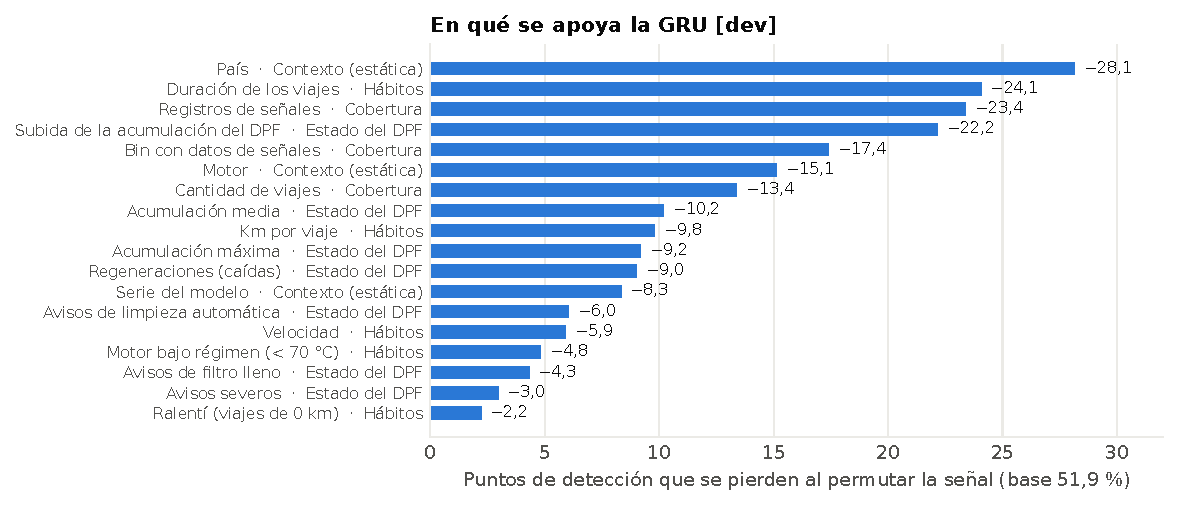
\includegraphics[width=\textwidth]{figuras/permutacion.pdf}
\caption{Caída de la detección media al 5–20\,\% al permutar cada señal en la validación (dev, semilla 42,
repetición 0; detección base 51,9\,\%). Las caídas no se suman por familia: permutar una señal sola no es
esconder la familia.}
\label{fig:permutacion}
\fuente{\repo{experiments/\allowbreak{}explain-gru-final/\allowbreak{}units.csv}; \repo{configs/\allowbreak{}explain\_gru\_final.yaml}
(\repo{scripts/\allowbreak{}explain\_perm\_seq.py}).}
\end{figure}

\begin{itemize}
  \item \textbf{Hábitos}: la duración de los viajes es el que más pesa (−24,1 puntos), por delante de km por viaje
    (−9,8), velocidad (−5,9), motor bajo régimen (−4,8) y ralentí (−2,2).
  \item \textbf{Estado del filtro}: cuánto sube la acumulación (−22,2), su nivel medio (−10,2) y máximo (−9,2), y
    las regeneraciones (−9,0).
  \item \textbf{Contexto}: el país pesa más que cualquier señal (−28,1), y el motor −15,1. Es coherente con la celda
    como piso: el riesgo no es el mismo en todos los mercados.
  \item \textbf{Cobertura}: cuántos registros y viajes hay en cada tramo (−23,4 y −13,4). Que un tramo tenga datos
    o no también informa.
\end{itemize}
La lectura física es la del DPF: viajes cortos que no dejan terminar la regeneración y hollín que se acumula. No le
dimos ninguna regla del filtro: esa relación la aprendió de los datos.

\textbf{2 · Por qué este auto} (para el conductor y el concesionario). La GRU no tiene atribución por auto, y 7 de
sus 15 canales son el estado del propio filtro, que no es algo que el conductor pueda cambiar. Por eso el porqué
que se comunica \emph{no} es lo que usó el modelo, sino una comparación descriptiva:
\begin{itemize}
  \item el promedio de los cortes que dispararon la alerta se compara con la mediana de los autos sanos de
    desarrollo del mismo mercado;
  \item un hábito “se aparta” si supera al 75\,\% de esos sanos hacia el lado riesgoso, y se nombran hasta tres;
  \item \textbf{solo se nombran hábitos accionables cuyo efecto esperado coincide con la física del DPF}, de una
    lista cerrada antes de mirar los datos. Síntomas (nivel del filtro, regeneraciones, avisos, aceite, consumo) y
    contexto (mercado, odómetro) nunca llegan al conductor: van al taller.
\end{itemize}

El criterio físico viene de la explicabilidad del finalista de la entrega 1 (SHAP sobre survival stacking,
reconstruido bit a bit): 10 de los 15 hábitos accionables con hipótesis física coincidían con la física del DPF;
cuatro iban al revés (por ejemplo, viajes más largos asociados a más riesgo) y quedaron fuera del texto al cliente
(\repo{f4-explicabilidad-k2.md}). Por eso el texto dice “comparado con autos sanos de tu zona”, nunca “porque”: el
verificador rechaza el lenguaje causal.

\subsubsection{El pitch}
\label{sec:pitch}

El pitch cuenta la misma historia que este informe, en siete bloques y 29 minutos, y con los mismos números
(tabla~\ref{tab:pitch}). El hilo es un usuario común, “nuestro conductor”: hace viajes cortos en la ciudad, su
filtro se tapa sin que nadie lo note, y al final de la historia recibe el aviso a tiempo.

\begin{table}[H]
\centering
\caption{La estructura del pitch.}
\label{tab:pitch}
\scriptsize
\begin{tabularx}{\textwidth}{@{}>{\raggedright\arraybackslash}p{2.6cm}>{\raggedright\arraybackslash}X>{\raggedright\arraybackslash}p{4.8cm}@{}}
\toprule
Bloque & Pregunta que responde & Frase ancla \\
\midrule
1 · El problema & ¿Por qué le importa a Ford? & “El auto avisa cuando el filtro ya no da más. Y el cliente se entera solo.” \\
2 · Los datos & ¿Qué hay en la telemetría y qué trampas tenía? & “La forma de manejar deja huella meses antes.” \\
3 · El modelo & ¿Qué probamos, qué ganó y cuánto detecta? & “Casi 1 de cada 3, tres meses antes, con 5\,\% de falsas alarmas.” \\
4 · El producto & ¿Qué pasa después de la alerta? (agentes y demo en vivo) & “El modelo decide. El agente habla como una persona. El código cuida lo que dice.” \\
5 · Escalabilidad & ¿Cómo llega a un millón de autos? & “Un millón de autos, sin un sensor nuevo.” \\
6 · Costos & ¿Qué pierde el cliente hoy y cuánto cuesta evitarlo? & “Cada aviso a tiempo es un cliente que confía más en Ford.” \\
7 · Cierre & ¿Por qué es distinto y qué necesita de Ford? & “Del testigo en el tablero al aviso a tiempo.” \\
\bottomrule
\end{tabularx}
\fuente{\repo{docs/\allowbreak{}pitch/\allowbreak{}presentacion-contenido.md}; deck en \repo{docs/\allowbreak{}pitch/\allowbreak{}deck/\allowbreak{}index.html}.}
\end{table}

Las reglas para citar números son las mismas en el deck y acá: toda detección al lado del azar; el resultado en test
y en rango; [test] y [dev] marcados; la anticipación como margen y no como pronóstico; nada de accuracy; y los
límites dichos antes de que los pregunten.
